\documentclass[tikz]{standalone}

\begin{document}
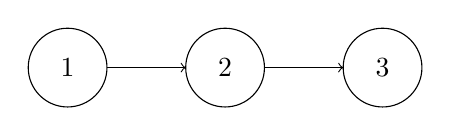
\begin{tikzpicture}
  \node[circle,
    draw = black,
    fill = white,
    minimum size = 1cm] (r) at (0,0) {1};
  \node[circle,
    draw = black,
    fill = white,
    minimum size = 1cm] (r) at (2,0) {2};
  \node[circle,
    draw = black,
    fill = white,
    minimum size = 1cm] (r) at (4,0) {3};

  \draw[->,thin,font=\Large] (0.5,0) -- (1.5,0);
  \draw[->,thin,font=\Large] (2.5,0) -- (3.5,0);
\end{tikzpicture}
\end{document}